\chapter{Ergebnisse}

Zunächst testen wir, wie gut welche Art von Output während Trainings- und Testphase abschneidet. Dazu vergleichen wir die Performance unter Variation des Outputs mit den jeweils drei entsprechenden Datensätzen. 

Anschließend integrieren wir das Netz in den DuckieTown-Simulator und bewerten die tatsächliche Performance in einer Validierungsphase.

\section{Training und Test}

Wie zu erwarten ist der Fehler des Netzes stark abhängig von der Verteilung der Trainingsdaten. So ergab sich in allen Fällen ein höherer Fehler, je größer der Anteil an Zufallsposen im Datensatz. 

\subsection{2D-Pose}

Beim Training auf eine \acs{2d}-Pose fällt auf, dass das Schätzen des Winkels $\theta$ eine größere Herausforderung darstellt, als das Schätzen der Distanz $d$. \ref{2d-poses-mse} zeigt, dass bei dem Training mit Daten mit hohem Anteil an Zufallsposen (Datensatz ``\acs{pd}-Rand'' in den Farben Grün und Lila) das Netz etwa ab der zehnten Epoche überstimmt ist. Im Vergleich mit den absoluten Fehlern der einzelnen Dimensionen in \ref{2d-poses-mae-d} und \ref{2d-poses-mae-a}, ist festzustellen, dass die Überstimmung vor allem auf Schwierigkeiten mit dem Schätzen des Winkels $\theta$ zurückzuführen ist.

Bei dem Schätzen der Distanz $d$ ist selbst mit dem ``\acs{pd}-Rand'' Datensatz in Epoche 50 die Überstimmung des Netzes minimal, wie in \ref{2d-poses-mae-d} zu sehen ist.


\begin{figure}[H]
	\centering
		\begin{tabular}[t]{|l|r|r|r|}
			\hline
			Datensatz & MSE & MAE $d$ & MAE $\theta$ \\
			\hline
			PD & 8.164 & 1.404 & 1.784 \\
			\hline
			PD-Rand & 274.2 & 8.312 & 12.61 \\
			\hline
			PD + PD-Rand & 143.8 & 5.353 & 8.036 \\
			\hline
		\end{tabular}
	\caption{Performance der \acs{2d}-Posenschätzung auf Testdaten}
	\label{2d-pose-performance}
\end{figure}

\begin{figure}[H]
	\centering
	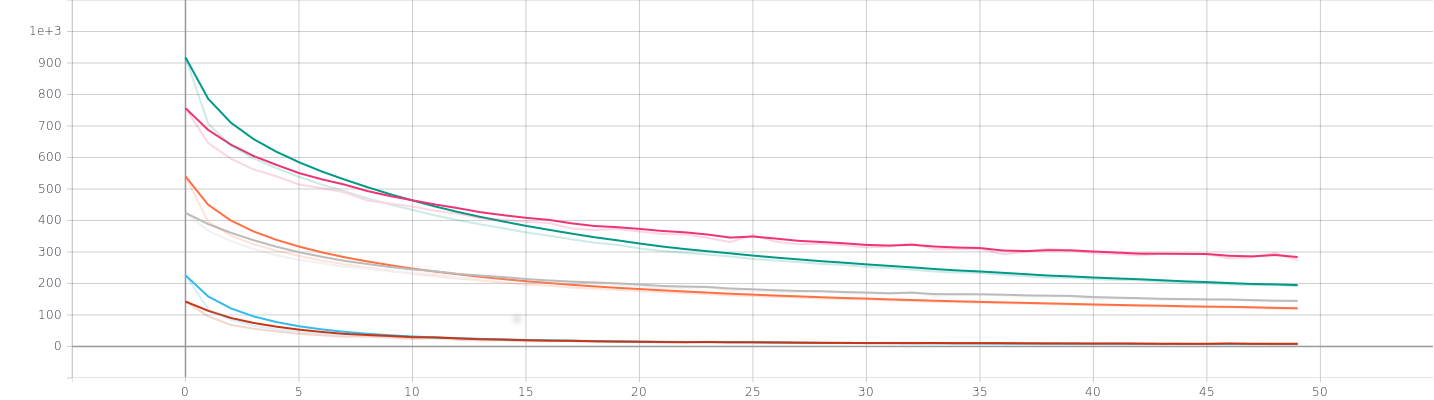
\includegraphics[width=\linewidth]{kapitel5/images/tensorboard/single-loss/Loss-single-loss.png}
	\caption{\acs{mse} mit \acs{2d}-Posenschätzung}
	\label{2d-poses-mse}
\end{figure}

\begin{figure}[H]
	\centering
	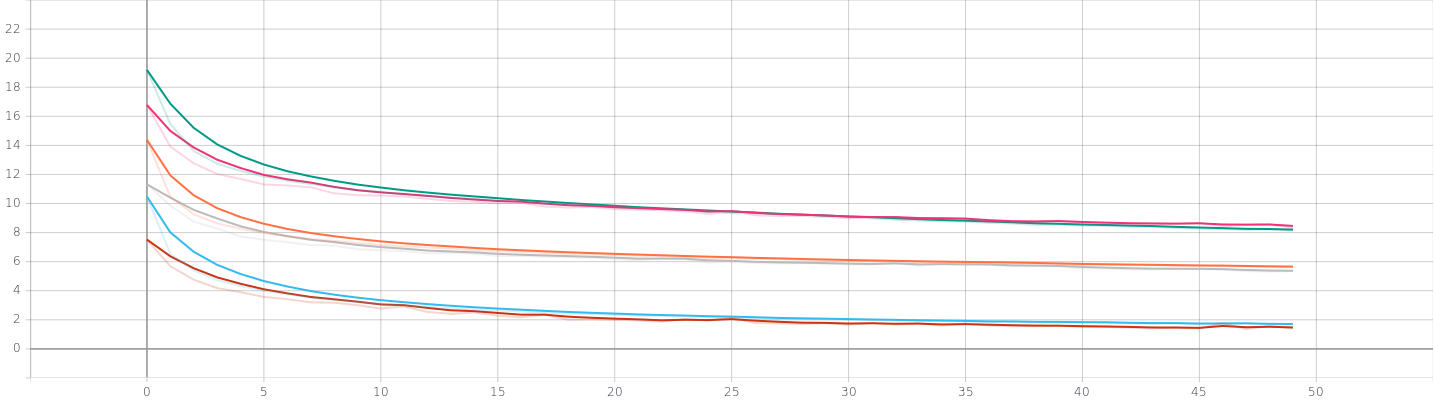
\includegraphics[width=\linewidth]{kapitel5/images/tensorboard/single-loss/Mean_Abs_Error_d-single-loss.png}
	\caption{\acs{mae} der Distanz mit \acs{2d}-Posenschätzung}
	\label{2d-poses-mae-d}
\end{figure}

\begin{figure}[H]
	\centering
	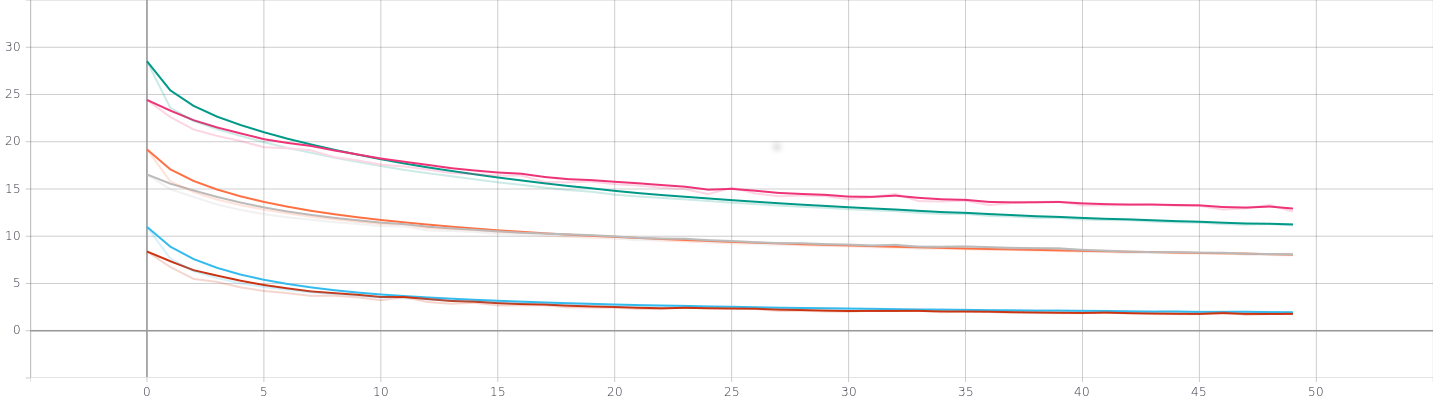
\includegraphics[width=\linewidth]{kapitel5/images/tensorboard/single-loss/Mean_Abs_Error_a-single-loss.png}
	\caption{\acs{mae} des Winkels mit \acs{2d}-Posenschätzung}
	\label{2d-poses-mae-a}
\end{figure}

\subsection{1D-Pose}

Das Entfernen des Winkels aus dem Zustandsvektor bringt eine leichte Verbesserung der Performance auf allen Datensätzen mit sich (siehe \ref{1d-pose-performance} und \ref{2d-pose-performance}). 

\begin{figure}[H]
	\centering
	\begin{tabular}[t]{|l|r|r|}
		\hline
		Datensatz & MSE & MAE $d$ \\
		\hline
		PD & 3.423 & 1.104 \\
		\hline
		PD-Rand & 115.4 & 6.73 \\
		\hline
		PD + PD-Rand & 60.0 & 4.364 \\
		\hline
	\end{tabular}
	\caption{Performance der \acs{1d}-Posenschätzung auf Testdaten}
	\label{1d-pose-performance}
\end{figure}

\begin{figure}[H]
	\centering
	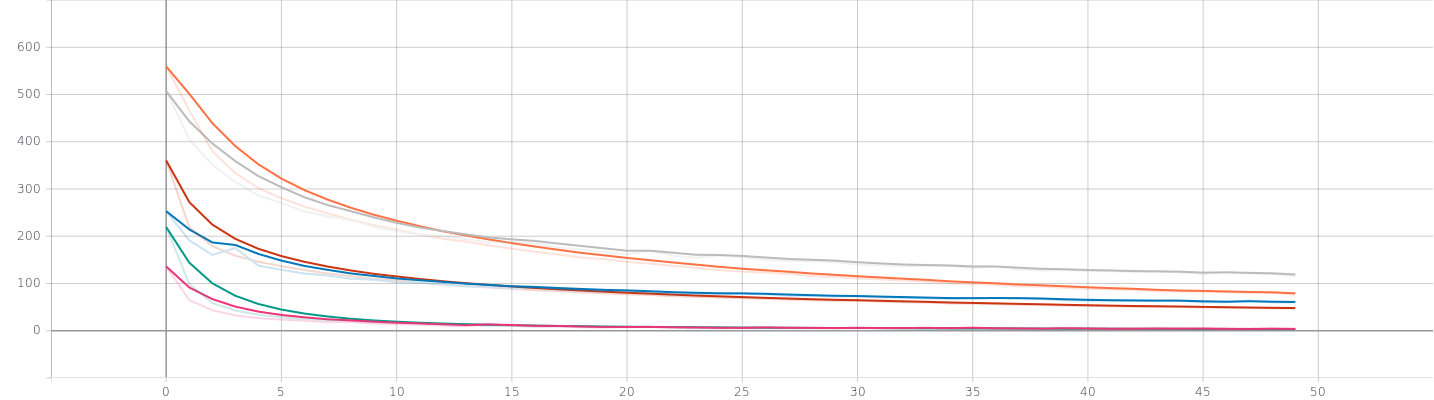
\includegraphics[width=\linewidth]{kapitel5/images/tensorboard/d-only/Loss-d-only.png}
	\caption{\acs{mse} der Distanz mit \acs{1d}-Posenschätzung}
	\label{1d-poses-mse-d}
\end{figure}

Allerdings führt die Reduktion auf das Schätzen des Distanzwertes allein zu einer stärkeren Überstimmung des Netzes. In \ref{1d-poses-mse-d} ist erkennbar, dass sowohl bei dem Training mit dem ``\acs{pd}-Rand'' (hier in Orange für die Trainingsdaten und Grau für die Testdaten), als auch mit dem ``\acs{pd} + \acs{pd}-Rand'' Datensatz (Rot für Training und Blau für Test), das Netz spätestens ab Epoche 15 überstimmt ist.

\subsection{Steuerbefehl durch Expertensystem}

% \begin{figure}[H]
% 	\centering
% 	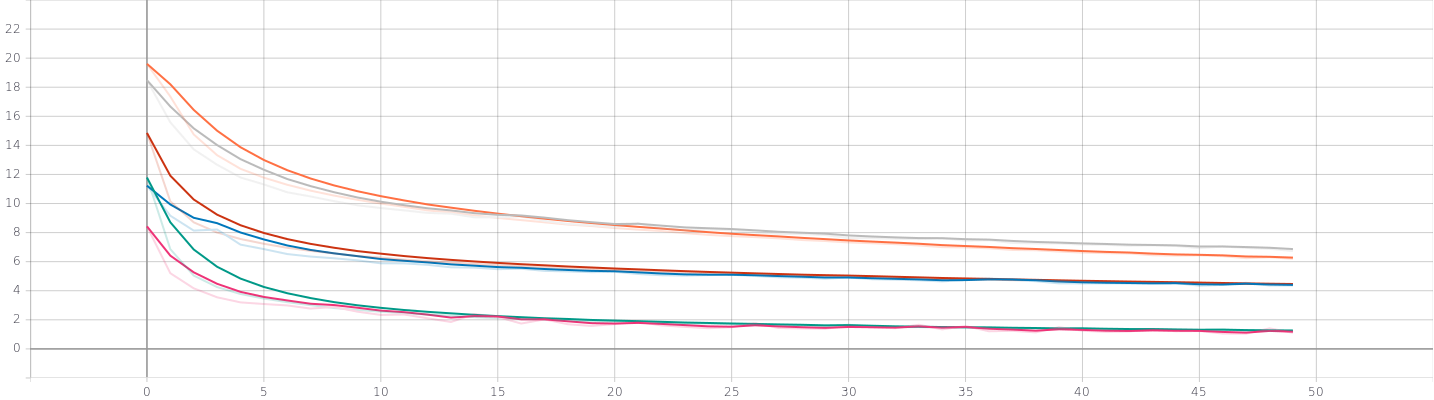
\includegraphics[width=\linewidth]{kapitel5/images/d-only/Mean_Abs_Error_d-d-only.png}
% 	\caption{MAE der Distanz mit 1D-Posenschätzung}
% 	\label{1d-poses-mae-d}
% \end{figure}

Wie zuvor zeigt sich auch hier, dass das Training mit hohem Anteil an Zufallsposen in den Daten zu einer Überstimmung des Netzes führt. So bilden sich deutliche Lücken zwischen der Performance auf Trainings- und Testdaten auf den Datensätzen ``Expert-Rand'' (Test Grau und Training Orange) und ``Expert + Expert-Rand'' (Test Blau und Training Rot) in \ref{expert-mse-omega}.


\begin{figure}[H]
	\centering
	\begin{tabular}[t]{|l|r|r|}
		\hline
		Datensatz & MSE & MAE $\omega$ \\
		\hline
		Expert & 0.00536 & 0.04214 \\
		\hline
		Expert-Rand & 0.11 & 0.205 \\
		\hline
		Expert + Expert-Rand & 0.057 & 0.1322 \\
		\hline
	\end{tabular}
	\caption{Performance der Schätzung eines Steuerbefehls auf Testdaten}
	\label{expert-performance}
\end{figure}

\begin{figure}[H]
	\centering
	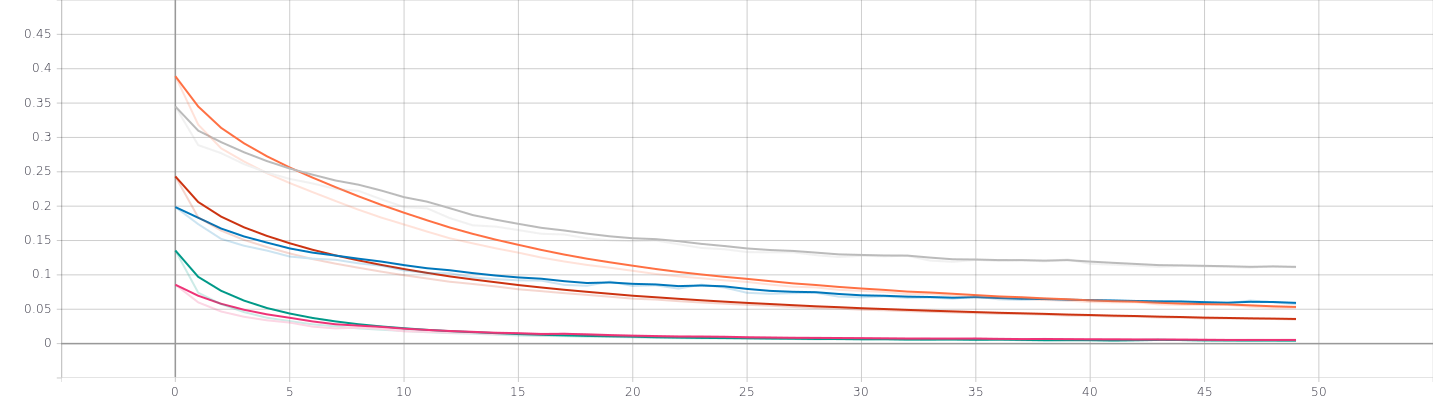
\includegraphics[width=\linewidth]{kapitel5/images/tensorboard/expert/Loss-expert.png}
	\caption{\acs{mse} der Winkelgeschwindigkeit mit Expertenbefehl}
	\label{expert-mse-omega}
\end{figure}

% \begin{figure}[H]
% 	\centering
% 	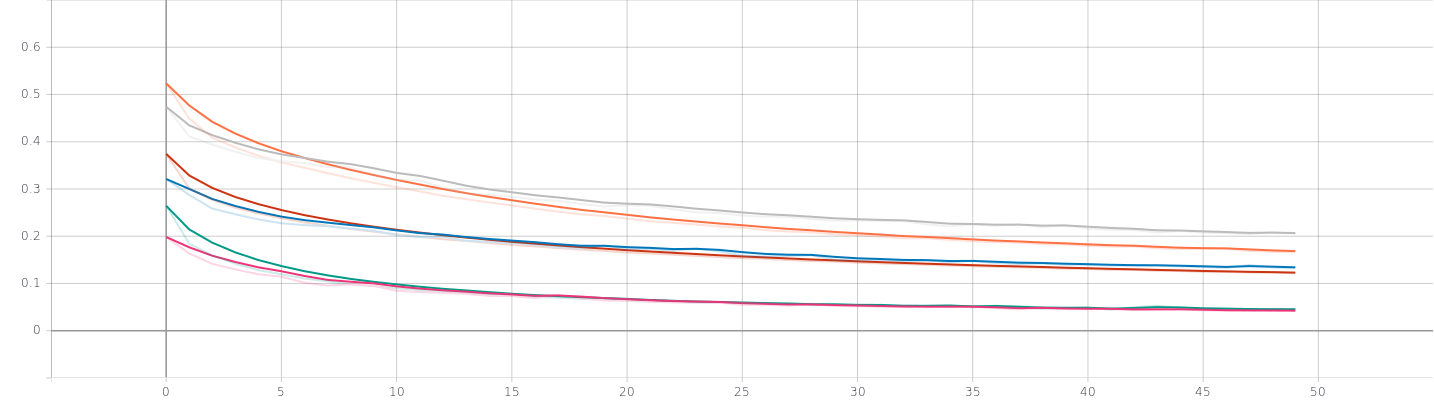
\includegraphics[width=\linewidth]{kapitel5/images/expert/Mean_Abs_Error_omega-expert.png}
% 	\caption{MAE der Winkelgeschwindigkeit mit Expertenbefehl}
% 	\label{expert-mae-omega}
% \end{figure}

\section{Validierung}

Die Validierung besteht aus der Integration des Netzes in den Simulator, wobei dieses selbst die Kontrolle übernimmt. Die Steuerung erfolgt dabei in Abhängigkeit von dem Output des Netzes. Im Falle des \acs{2d}-Posen-Netzes über einen einfachen \acs{pd}-Regler mit $d$ als Fehler und $\theta$ als Ableitung des Fehlers (siehe \ref{pd-drive-example}). Das \acs{1d}-Posen-Netz hält den Distanzwert über einen vollständigen und sorgfältig eingestellten \acs{pid}-Regler. Das Experten-Netz steuert den Agenten direkt über den inferierten Steuerbefehl.

Im Gegensatz zur Trainings- und Testphase ist bei der Integration in den Simulator die Verteilung der Werte mit denen das Netz konfrontiert wird abhängig davon, wie gut dieses die Spur halten kann. Dies ist wiederum abhängig davon, wie gut die letzten Werte geschätzt worden sind.

Wir lassen die Netze jeweils 100000 \texttt{step()}-Aufrufe des Simulators fahren, was bei einer Bildrate von 30 Bildern pro Sekunde einer Fahrdauer von etwa einer Stunde entspricht.\\

\subsection{2D-Pose}

Im ersten Fall des \acs{2d}-Posen-Netzes schnitt das Netz, welches mit dem ``\acs{pd}-Rand''-Datensatz und damit dem höchsten Anteil an Zufallsposen trainiert wurde, in Sachen Crashes pro Schritte am besten ab. Auffällig ist, dass das Training mit ``\acs{pd}-Concat'' zwar zu einen besseren durchschnittlichen Fehler führte, was auch mit dem doppelt so großen Umfang des Datensatzes zu erklären ist, jedoch nicht zu der geringsten Anzahl an Crashes.  

\begin{table}[H]
	\centering
	\begin{tabular}[t]{|c|l|r|r|r|}
		\hline
		& \textbf{Kacheltyp} & \textbf{MAE $d$, $\theta$} & \textbf{n} & Crashes \\
		\hline
		\multirow{4}{*}{PD} 
		& Alle
		& 12.59, 20.41
		& 100000
		& \multirow{4}{*}{790}\\
		\cline{2-4}
		& Gerade
		&  9.76, 13.79
		& 53433
		&\\
		\cline{2-4}
		& Linkskurve
		& 16.70,  35.28
		& 20311
		&\\
		\cline{2-4}
		& Rechtskurve
		& 23.78, 37.95 
		& 4728
		&\\
		\cline{2-4}
		& 3-Wege
		&  13.27, 18.95
		& 21528
		&\\
		\hline
		\multirow{4}{*}{PD-Rand} 
		& Alle
		& 11.63, 17.19
		& 100000
		& \multirow{4}{*}{485}\\
		\cline{2-4}
		& Gerade
		&  9.67, 13.08
		& 55325 & \\
		\cline{2-4}
		& Linkskurve
		& 14.38, 26.80
		& 18513
		&\\
		\cline{2-4}
		& Rechtskurve
		& 16.44, 31.53
		& 3796
		&\\
		\cline{2-4}
		& 3-Wege
		& 13.36, 16.97
		& 22366
		&\\
		\hline
		\multirow{4}{*}{PD-Concat} 
		& Alle
		& 10.62, 16.37
		& 100000
		& \multirow{4}{*}{592}\\
		\cline{2-4}
		& Gerade
		& 7.67, 11.04
		& 49792
		&\\
		\cline{2-4}
		& Linkskurve
		& 13.73, 23.53
		& 24695
		&\\
		\cline{2-4}
		& Rechtskurve
		& 17.59, 29.68
		& 5163
		&\\
		\cline{2-4}
		& 3-Wege
		& 12.28, 17.35
		& 20350
		&\\
		\hline
	\end{tabular}
	\caption{Validierung des 2D-Posen-Netzes}
	\label{2d-validation}
\end{table}

In der Verteilung der Werte, mit welchen das Netz während der Integration konfrontiert wurde, ist das bessere Fahrverhalten des mit dem ``\acs{pd}-Rand''-Datensatz trainierten Netzes ebenfalls erkennbar. So liegt der Schwerpunkt der Entfernungswerte eher nahe 20, was der Mitte der rechten Fahrspur entspricht. Auch die Winkel streuen eher um 0, was eine gute Orientierung während des Fahrens anzeigt.

Die anderen beiden Varianten befanden sich während der Fahrt eher auf der gegenüberliegenden Fahrspur (Schwerpunkt der Distanzwerte um 60) und neigten zu einer linkslastigen Orientierung (Schwerpunkt der Winkel unter 0).

\begin{figure}[H]
	\centering
	\begin{subfigure}[h]{0.5\textwidth}
		\centering
		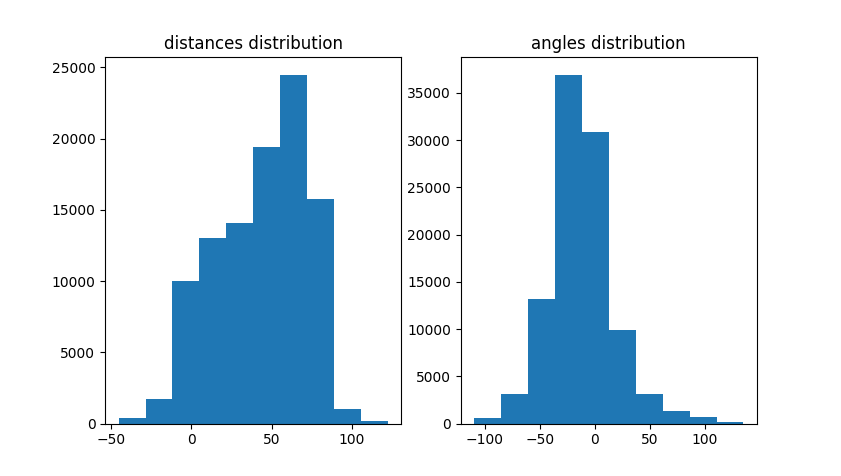
\includegraphics[width=\linewidth]{kapitel5/images/eval/single-loss/pd-distr.png}
		\caption{``PD''}
		\label{2d-pd-val-distr}
	\end{subfigure}%
	\begin{subfigure}[h]{0.5\textwidth}
		\centering
		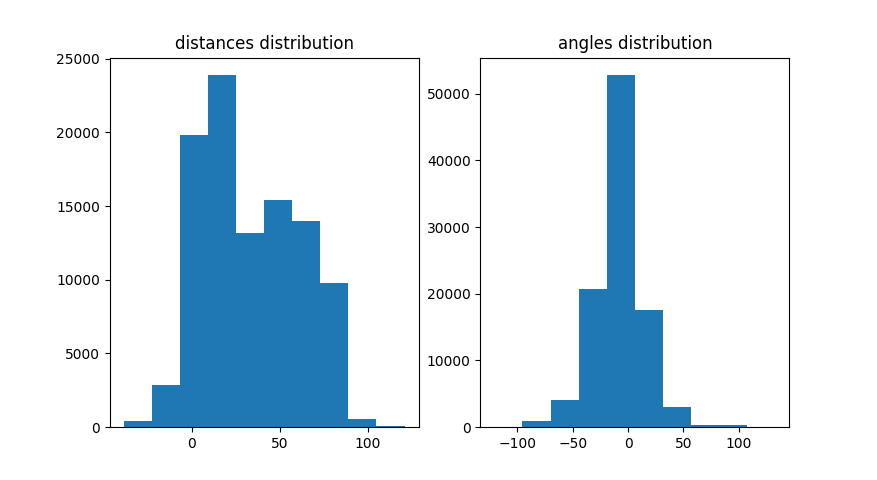
\includegraphics[width=\linewidth]{kapitel5/images/eval/single-loss/pd-rand-distr.png}
		\caption{``PD-Rand''}
		\label{2d-pd-rand-val-distr}
	\end{subfigure}
	\begin{subfigure}[h]{0.5\textwidth}
		\centering
		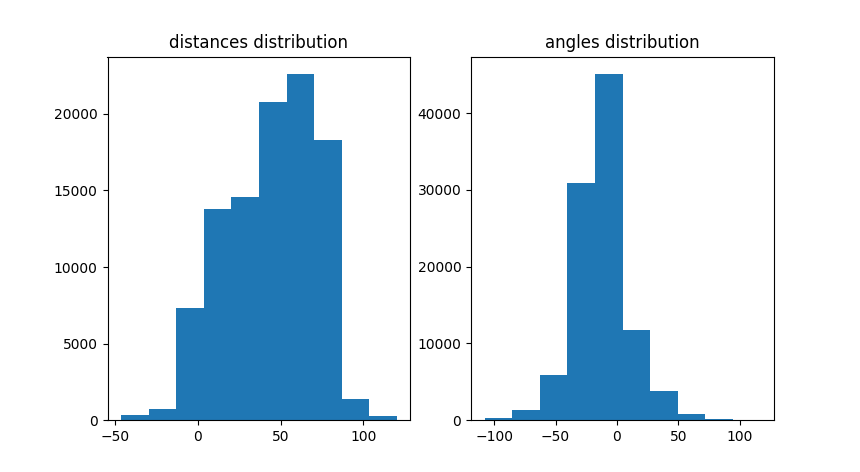
\includegraphics[width=\linewidth]{kapitel5/images/eval/single-loss/pd-concat-distr.png}
		\caption{``PD-Concat''}
		\label{2d-pd-concat-val-distr}
	\end{subfigure}
	\caption{Verteilungen der erlebten Werte während der Validierung des 2D-Netzes}
	\label{2d-val-distr}
\end{figure}

\subsection{1D-Pose}



\begin{table}[H]
	\centering
	\begin{tabular}[t]{|c|l|r|r|r|}
		\hline
		& \textbf{Kacheltyp} & \textbf{MAE $d$} & \textbf{n} & Crashes \\
		\hline
		\multirow{4}{*}{PD} 
		& Alle
		& 5.32
		& 100000
		& \multirow{4}{*}{1}\\
		\cline{2-4}
		& Gerade
		&  3.09
		& 45990
		&\\
		\cline{2-4}
		& Linkskurve
		& 9.77
		& 34287
		&\\
		\cline{2-4}
		& Rechtskurve
		& 7.85
		& 4403
		&\\
		\cline{2-4}
		& 3-Wege
		&  1.34
		& 15320
		&\\
		\hline
		\multirow{4}{*}{PD-Rand} 
		& Alle
		& 14.44
		& 100000
		& \multirow{4}{*}{27}\\
		\cline{2-4}
		& Gerade
		&  9.73
		& 7974
		& \\
		\cline{2-4}
		& Linkskurve
		& 13.01
		& 1324
		&\\
		\cline{2-4}
		& Rechtskurve
		& 14.83
		& 89228
		&\\
		\cline{2-4}
		& 3-Wege
		& 17.22
		& 1474
		&\\
		\hline
		\multirow{4}{*}{PD-Concat} 
		& Alle
		& 8.37
		& 100000
		& \multirow{4}{*}{49}\\
		\cline{2-4}
		& Gerade
		& 6.36
		& 80467
		&\\
		\cline{2-4}
		& Linkskurve
		& 16.04
		& 9792
		&\\
		\cline{2-4}
		& Rechtskurve
		& 23.76
		& 4276
		&\\
		\cline{2-4}
		& 3-Wege
		& 12.19
		& 5465
		&\\
		\hline
	\end{tabular}
	\caption{Validierung des 1D-Posen-Netzes}
	\label{1d-validation}
\end{table}

\subsection{Expertenbefehl}

\begin{table}[H]
	\centering
	\begin{tabular}[t]{|c|l|r|r|r|}
		\hline
		& \textbf{Kacheltyp} & \textbf{MAE $\omega$} & \textbf{n} & Crashes \\
		\hline
		\multirow{4}{*}{Expert} 
		& Alle
		& 0.096
		& 100000
		& \multirow{4}{*}{2}\\
		\cline{2-4}
		& Gerade
		&  0.064
		& 49249
		&\\
		\cline{2-4}
		& Linkskurve
		& 0.162
		& 31399
		&\\
		\cline{2-4}
		& Rechtskurve
		& 0.126
		& 3002
		&\\
		\cline{2-4}
		& 3-Wege
		&  0.061
		& 16350
		&\\
		\hline
		\multirow{4}{*}{Expert-Rand} 
		& Alle
		& 0.506
		& 100000
		& \multirow{4}{*}{311}\\
		\cline{2-4}
		& Gerade
		&  0.486
		& 48791
		& \\
		\cline{2-4}
		& Linkskurve
		& 0.573
		& 28062
		&\\
		\cline{2-4}
		& Rechtskurve
		& 0.715
		& 1657
		&\\
		\cline{2-4}
		& 3-Wege
		& 0.446
		& 21490
		&\\
		\hline
		\multirow{4}{*}{Expert-Concat} 
		& Alle
		& 0.150
		& 100000
		& \multirow{4}{*}{34}\\
		\cline{2-4}
		& Gerade
		& 0.117
		& 47454
		&\\
		\cline{2-4}
		& Linkskurve
		& 0.212
		& 31424
		&\\
		\cline{2-4}
		& Rechtskurve
		& 0.199
		& 3888
		&\\
		\cline{2-4}
		& 3-Wege
		& 0.117
		& 17234
		&\\
		\hline
	\end{tabular}
	\caption{Validierung des Steuerbefehl-Netzes}
	\label{expert-validation}
\end{table}
